\chapter{Algorithm development}
Her finder vi to signaler og så vores ønske output. Vi skal finde den algorithme som giver det ønskede output. De to inputs kan være vores skubbede chirp eller vores simple arrayindekseret output. Det ønskede output er xcorr funktionen fra matlab
Vi skulle også gerne i det her punkt have fundet nogle krav - fx at vi bør bruge så og så mange samples eller vi skal bruge en bestemt frekvens / frekvens span















\section{Signals}
To determine which signal type which was most favourable to use we made a script in matlab which generated 3 signal types, here one signal without a delay and one with a delay. This way we can analyse which signals would return the sharpest spike when cross correlated.
\subsection{Chirp}
A chirp is a signal which starts at a particular frequency and then changes the frequency fluently until it ends at another frequency.\\
Below is shown the code generating a chirp from 8kHz to 10kHz, then making a delayed version of this signal and lastly cross-correlating these signals.\\
\begin{lstlisting}[language=Matlab,frame=lrtb,label=Matlab Code for Chirp Cross-correlation]
Fs=48000;                                       % Sample frequency
t = [0:1/Fs:1];                                 % Timeinterval and length
Frq1=8000;                                      % Start frequency for chirp
Frq2=10000;                                     % End frequency for chirp
delay = 2000;                                   % Signal Delay
Chirp_signal=chirp(t,Frq1,1,Frq2);              % Chirp signal generation
Chirp_delayed=[zeros(1,delay) Chirp_signal];    % Chip delay generation
Chirp_xcorr=xcorr(Chirp_signal,Chirp_delayed);  % Cross-correlation
\end{lstlisting}
Below is the plot of the cross-correlation. It shows clearly where the to signal overlap.\\
\begin{figure}[H]
\begin{minipage}[b]{0.49\linewidth}
\centering
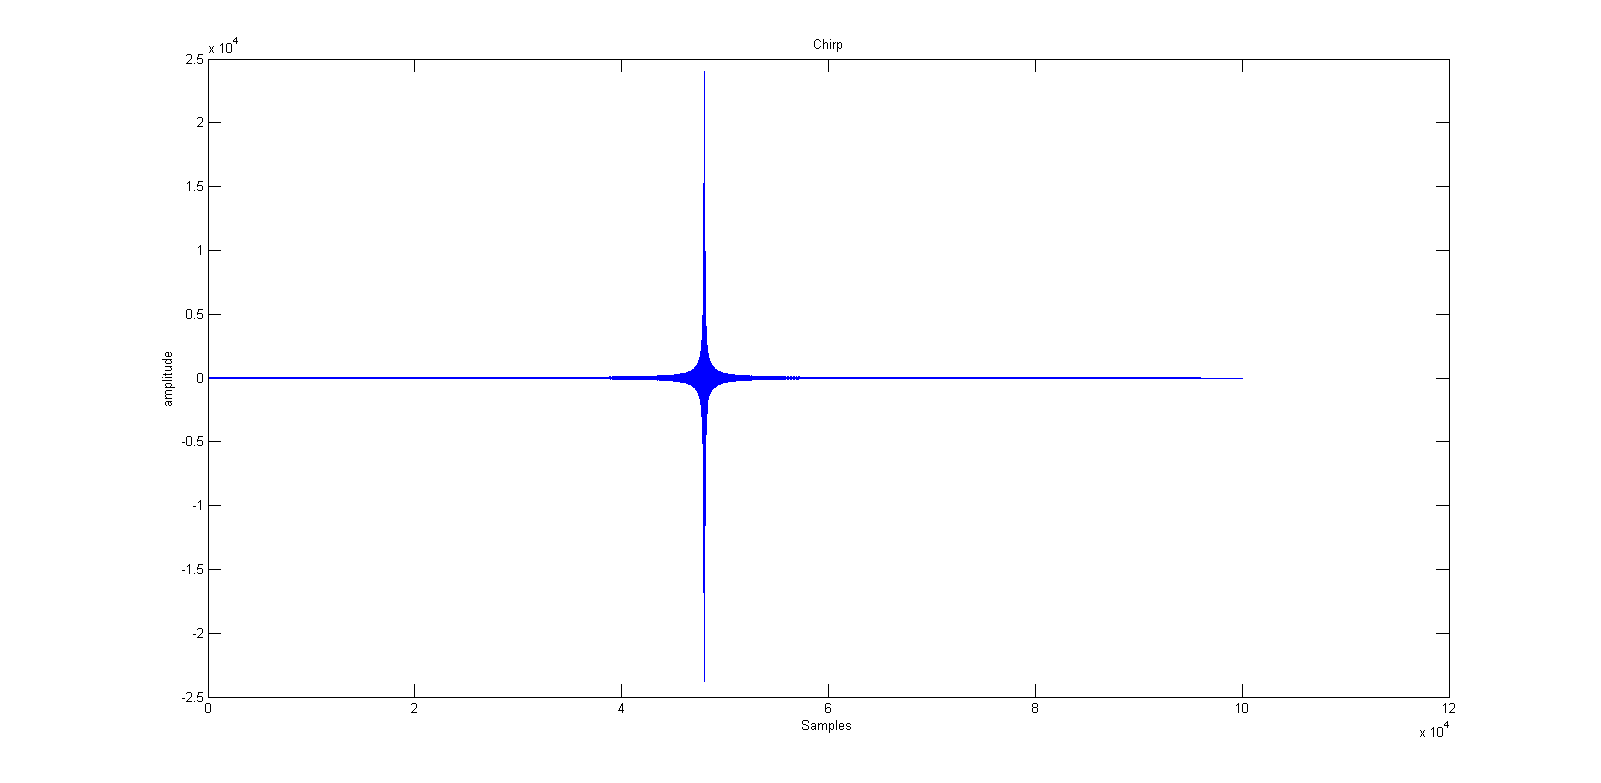
\includegraphics[width=1\textwidth]{billeder/chirp_xcorr_fig}
\caption{Chirp Cross-correlation}
\label{fig:figure1}
\end{minipage}
\hspace{0.5cm}
\begin{minipage}[b]{0.49\linewidth}
\centering
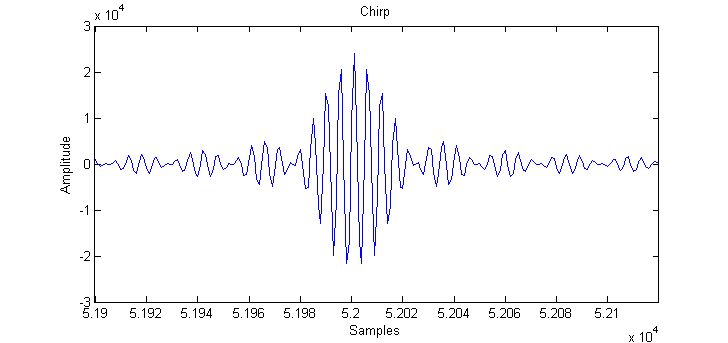
\includegraphics[width=1\textwidth]{billeder/chirp_xcorr_fig_zoom}
\caption{zoomed}
\label{fig:figure2}
\end{minipage}
\end{figure}
The Chirp seems like a solid signal to transmit. Since there exist a very specific area where it is clear the signals perfectly overlaps. The overlap shown above is centered around sample no. 52000 and spans around 10 samples.\\
This can easily be used to determine a somewhat precise distance. The distance of 10 samples @48kHz at the speed of sound is ~7cm.\\
Although matlab finds a precise sample for the max value we will have in mind that values close to the max is within the range of $\pm 3.5cm$.\\
\subsection{Sinusoid}
The initial thoughts about a sinusoid were mixed. Since a sinusoid overlaps more and more in periods we expect a triangle like cross-correlation. The sinus signals is treated the same way as the chirps in matlab and below is a plot of the cross-correlation.
\begin{figure}[H]
\begin{minipage}[b]{0.49\linewidth}
\centering
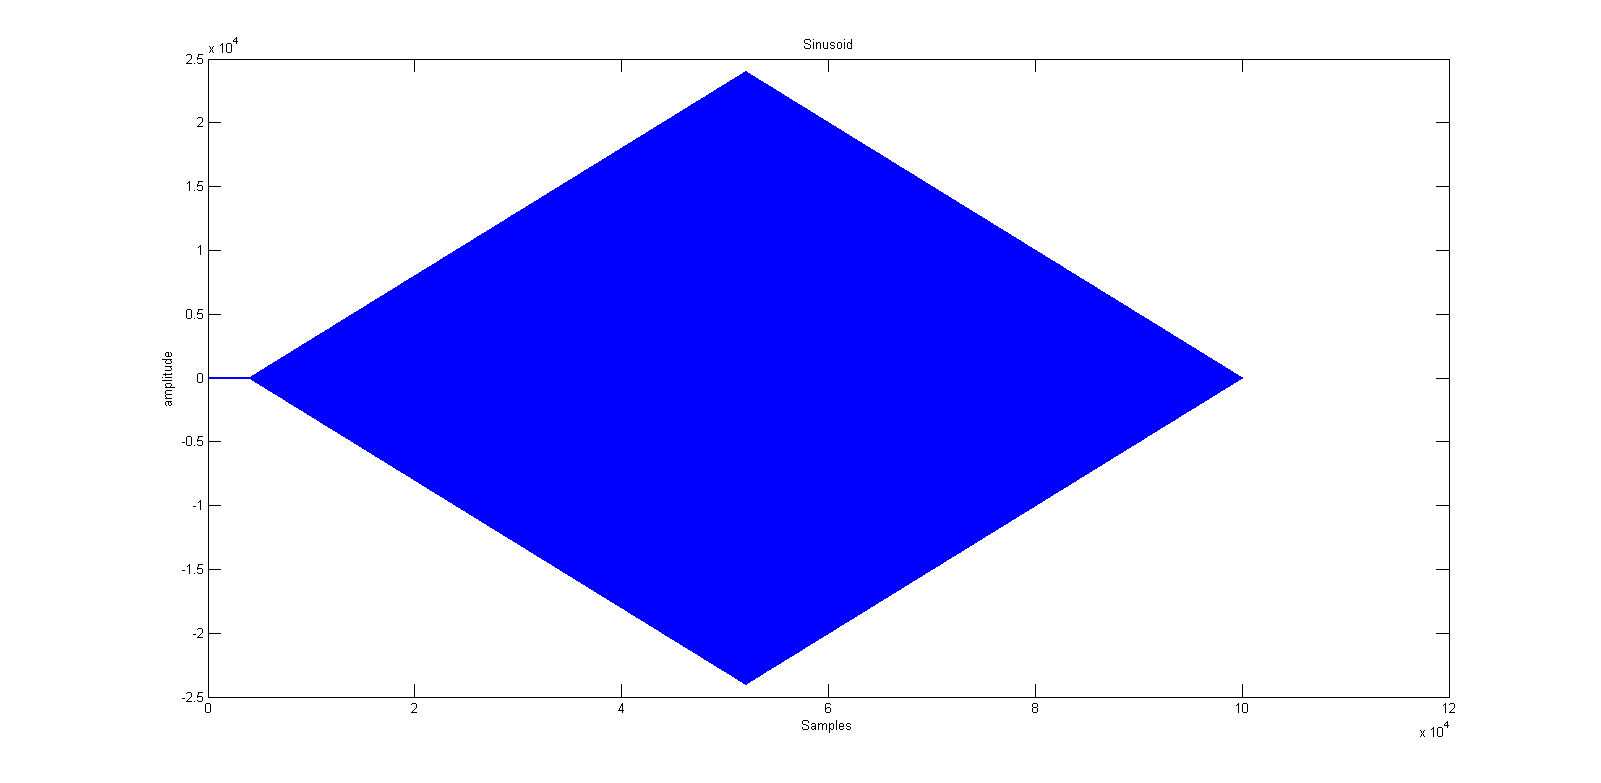
\includegraphics[width=1\textwidth]{billeder/sinus_xcorr_fig}
\caption{Sinusoid Cross-correlation}
\label{fig:figure1}
\end{minipage}
\hspace{0.5cm}
\begin{minipage}[b]{0.49\linewidth}
\centering
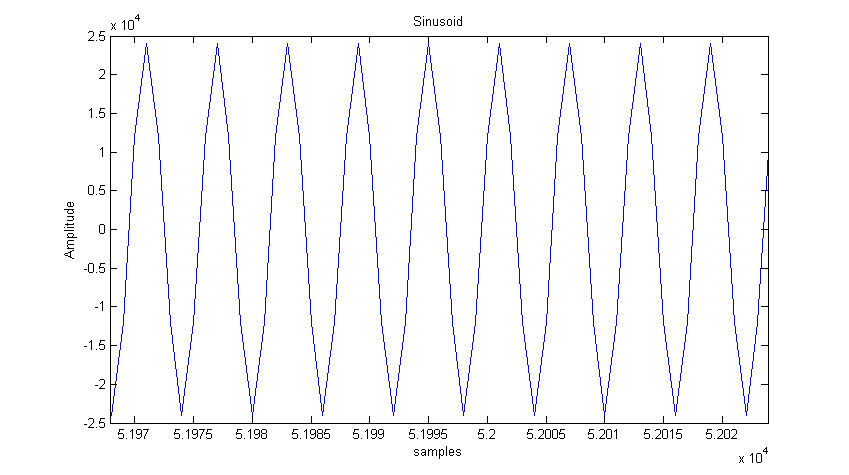
\includegraphics[width=1\textwidth]{billeder/sinus_xcorr_fig_zoom}
\caption{zoomed}
\label{fig:figure2}
\end{minipage}
\end{figure}
The zoomed plot is zoomed to the same window as the chirp signal. It is clear that the sinusoids peak isn't nearly as distinct as the chirp, hereby making the sinusoid signal less favourable. This also fits with our expectation since the sinusoid is very "simple" in shape compared to the chirp which is more unique.\\
\subsection{White noise}
Lastly we tried white noise. We expect this to be very distinct because the signal is very complex and consists of a lot of different frequencies. Therefore the signal will only overlay perfectly in one particular point. A noise signal was generated in matlab using the wgn() function. Below is a plot of the cross correlaltion.\\
\begin{figure}[H]
\begin{minipage}[b]{0.49\linewidth}
\centering
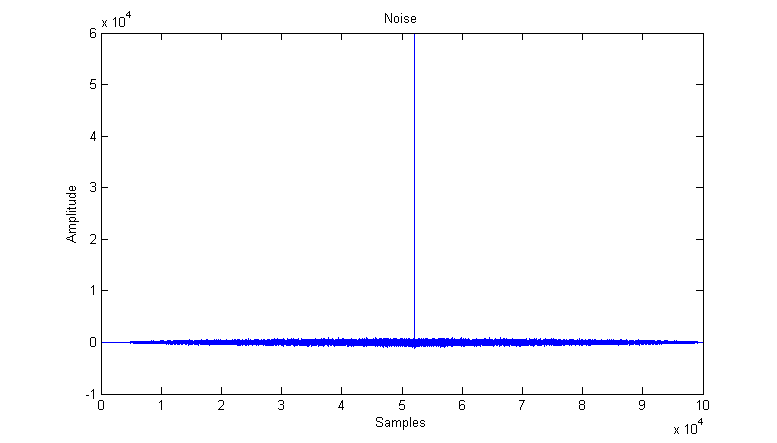
\includegraphics[width=1\textwidth]{billeder/noise_xcorr_fig}
\caption{Noise Cross-correlation}
\label{fig:figure1}
\end{minipage}
\hspace{0.5cm}
\begin{minipage}[b]{0.49\linewidth}
\centering
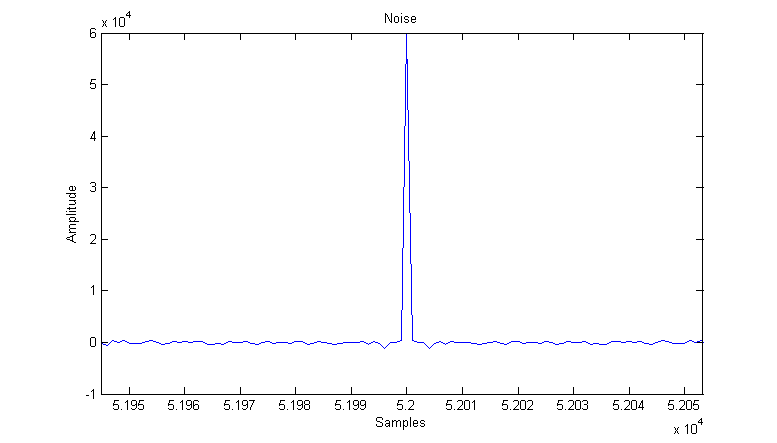
\includegraphics[width=1\textwidth]{billeder/noise_xcorr_fig_zoom}
\caption{zoomed}
\label{fig:figure2}
\end{minipage}
\end{figure}
As expected the noise was subject to a very sharp and distinct peak where the signals perfectly overlayed. The noise signals clearly seems like the best signal to transmit. The largest issue with the noise signal is that it is a very broad spectre. Since it is white noise it consists equally much of all signals.\\
\subsection{Robustness of signals}
%Her ligges der lidt støj ind over signalerne for at se hvor modstandsdygtige de er for støj.
As a last analysis of the signals we want to check the robustness of the signals. We want to do this by overlaying the generated signals with some noise. This is simply done in matlab by adding a noise signal to the original signal.\\
Before cross-correlating the signals an fft and a signal plot is made to ensure that the signals indeed have been overlayed with noise. Below is are these plots for the chirp.
\begin{figure}[H]
\begin{minipage}[b]{0.49\linewidth}
\centering
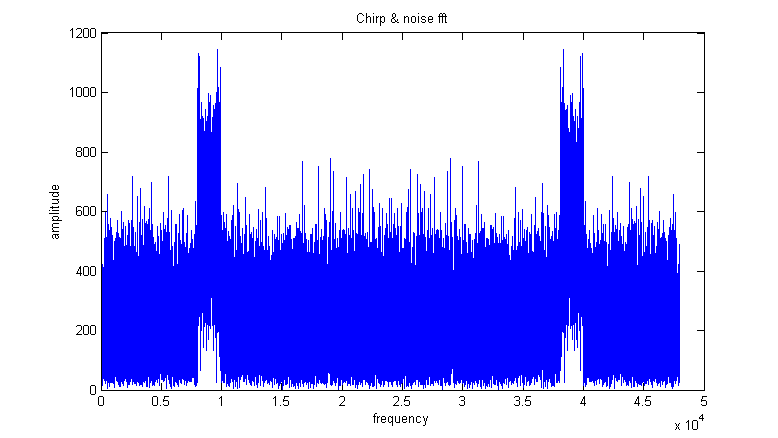
\includegraphics[width=1\textwidth]{billeder/chirp_noise_fft}
\caption{Chirp \& noise fft}
\label{fig:figure1}
\end{minipage}
\hspace{0.5cm}
\begin{minipage}[b]{0.49\linewidth}
\centering
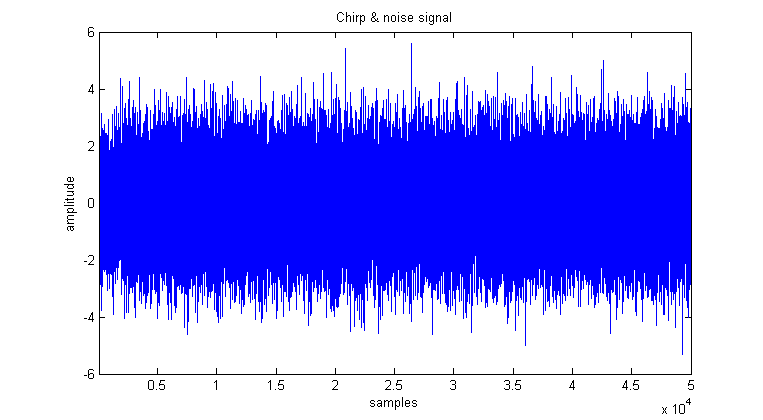
\includegraphics[width=1\textwidth]{billeder/chirp_noise_signal}
\caption{Chirp \& noise plot}
\label{fig:figure2}
\end{minipage}
\end{figure}
The fft plot shows that there is a lot of noise distributed over all frequencies but the original chirp is still present. The signal plot shows how much the chirp is disguised in the noise.\\
Below is a plot of the cross-correlation.
\begin{figure}[H]
\begin{minipage}[b]{0.49\linewidth}
\centering
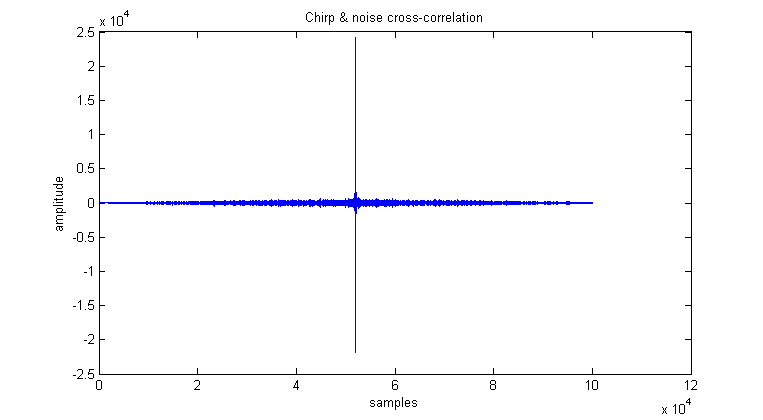
\includegraphics[width=1\textwidth]{billeder/chirp_noise_xcorr}
\caption{Chirp \& noise Cross-correlation}
\label{fig:figure1}
\end{minipage}
\hspace{0.5cm}
\begin{minipage}[b]{0.49\linewidth}
\centering
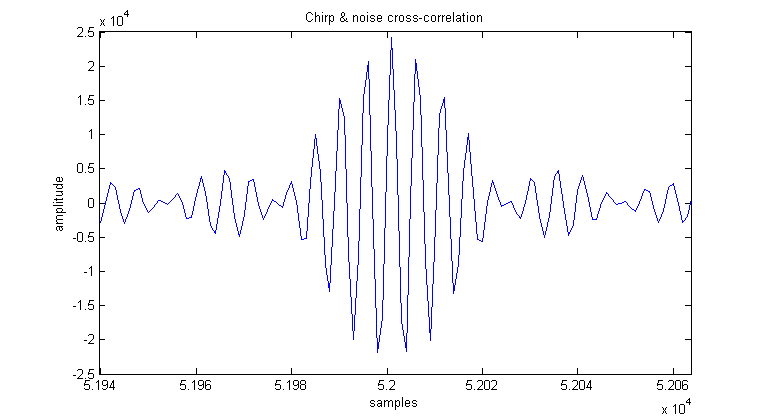
\includegraphics[width=1\textwidth]{billeder/chirp_noise_xcorr_zoom}
\caption{zoomed}
\label{fig:figure2}
\end{minipage}
\end{figure}
It is almost impossible to distinguish the noisy cross-correlation from the clean cross-correlation.\\